\setcounter{step}{0}
%------------------------------------------
% information doc
\subsection{IKEA torta}
%------------------------------------------

\begin{ingredient}
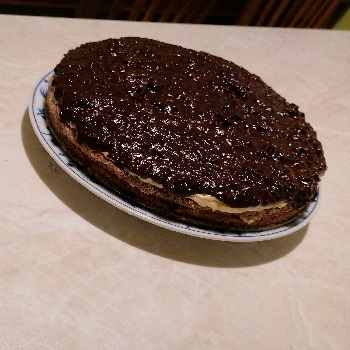
\includegraphics[height=5.5cm]{images/daim}
\def\portions{4}%
\textbf{{\normalsize Ingrediencie (\portions porcie):}}
%\vspace{0.5cm}
\begin{main}
\item
\end{main}
\begin{subingredient}{Korpus}
	\item 4 bielka
	\item 150g kryštálový cukor
	\item 150g mandle + 30g vlašské orechy
\end{subingredient}
\begin{subingredient}{Plnka}
	\item 1 LIDL Piknik
	\item 40g múka
	\item 1 vanilkový cukor
	\item 75g maslo
	\item 4 žĺtka
\end{subingredient}
\begin{subingredient}{Posyp}
	\item DAIM čokoláda / krokant
	\item 125g čokoláda
	\item 50ml smotana/mlieko
\end{subingredient}
\begin{subingredient}{Krokant}
	\item 50g kryštálový cukor
	\item 20g orechy
	\item 1ČL maslo + 30ml voda
\end{subingredient}
\end{ingredient}
\begin{recipe}
\textbf{{\normalsize Príprava:}}
\begin{enumerate}


\item{Pripravíme korpus:}
\begin{enumerate}
\item{bielka zmiešame s cukrom a vyšľaháme sneh}
\item{pridáme orechy a len rukou domiešame aby sneh nespadol}
\item{Dáme do vymúčenej formy a necháme piecť 35 minút na 175°}
\end{enumerate}

\item{Popri pečení pripravíme plnku:}

\begin{enumerate}
\item{Žĺtka a salko miešame nad parou}
\item{Pridáme cukor a múku}
\item{Po vychladnutí primiešame maslo}
\end{enumerate}

\item{Po upečení korpus rozrežeme a po vychladnutí naplníme plnkou}
\item{Na vrch dáme plnku a polejeme čokoládou zmiešanou s krokantom}


\end{enumerate}
\end{recipe}

%\begin{notes}

%\end{notes}
\clearpage	